\newcommand{\svcourse}{CST Part IA: Software Engineering and Security}
\newcommand{\svnumber}{1}
\newcommand{\svvenue}{Microsoft Teams}
\newcommand{\svdate}{2022-05-11}
\newcommand{\svtime}{15:00}
\newcommand{\svuploadkey}{CBd13xmL7PC1zqhNIoLdTiYUBnxZhzRAtJxv/ytRdM1r7qIfwMsxeVwM/pPcIo8l}

\newcommand{\svrname}{Dr Sam Ainsworth}
\newcommand{\jkfside}{oneside}
\newcommand{\jkfhanded}{yes}

\newcommand{\studentname}{Harry Langford}
\newcommand{\studentemail}{hjel2@cam.ac.uk}


\documentclass[10pt,\jkfside,a4paper]{article}

% DO NOT add \usepackage commands here.  Place any custom commands
% into your SV work files.  Anything in the template directory is
% likely to be overwritten!

\usepackage{fancyhdr}

\usepackage{lastpage}       % ``n of m'' page numbering
\usepackage{lscape}         % Makes landscape easier

\usepackage{verbatim}       % Verbatim blocks
\usepackage{listings}       % Source code listings
\usepackage{epsfig}         % Embed encapsulated postscript
\usepackage{array}          % Array environment
\usepackage{qrcode}         % QR codes
\usepackage{enumitem}       % Required by Tom Johnson's exam question header

\usepackage{hhline}         % Horizontal lines in tables
\usepackage{siunitx}        % Correct spacing of units
\usepackage{amsmath}        % American Mathematical Society
\usepackage{amssymb}        % Maths symbols
\usepackage{amsthm}         % Theorems

\usepackage{ifthen}         % Conditional processing in tex

\usepackage[top=3cm,
            bottom=3cm,
            inner=2cm,
            outer=5cm]{geometry}

% PDF metadata + URL formatting
\usepackage[
            pdfauthor={\studentname},
            pdftitle={\svcourse, SV \svnumber},
            pdfsubject={},
            pdfkeywords={9d2547b00aba40b58fa0378774f72ee6},
            pdfproducer={},
            pdfcreator={},
            hidelinks]{hyperref}


% DO NOT add \usepackage commands here.  Place any custom commands
% into your SV work files.  Anything in the template directory is
% likely to be overwritten!

\usepackage{fancyhdr}

\usepackage{lastpage}       % ``n of m'' page numbering
\usepackage{lscape}         % Makes landscape easier

\usepackage{verbatim}       % Verbatim blocks
\usepackage{listings}       % Source code listings
\usepackage{graphicx}
\usepackage{float}
\usepackage{epsfig}         % Embed encapsulated postscript
\usepackage{array}          % Array environment
\usepackage{qrcode}         % QR codes
\usepackage{enumitem}       % Required by Tom Johnson's exam question header

\usepackage{hhline}         % Horizontal lines in tables
\usepackage{siunitx}        % Correct spacing of units
\usepackage{amsmath}        % American Mathematical Society
\usepackage{amssymb}        % Maths symbols
\usepackage{amsthm}         % Theorems

\usepackage{ifthen}         % Conditional processing in tex

\usepackage[top=3cm,
            bottom=3cm,
            inner=2cm,
            outer=5cm]{geometry}

% PDF metadata + URL formatting
\usepackage[
            pdfauthor={\studentname},
            pdftitle={\svcourse, SV \svnumber},
            pdfsubject={},
            pdfkeywords={9d2547b00aba40b58fa0378774f72ee6},
            pdfproducer={},
            pdfcreator={},
            hidelinks]{hyperref}

\renewcommand{\headrulewidth}{0.4pt}
\renewcommand{\footrulewidth}{0.4pt}
\fancyheadoffset[LO,LE,RO,RE]{0pt}
\fancyfootoffset[LO,LE,RO,RE]{0pt}
\pagestyle{fancy}
\fancyhead{}
\fancyhead[LO,RE]{{\bfseries \studentname}\\\studentemail}
\fancyhead[RO,LE]{{\bfseries \svcourse, SV~\svnumber}\\\svdate\ \svtime, \svvenue}
\fancyfoot{}
\fancyfoot[LO,RE]{For: \svrname}
\fancyfoot[RO,LE]{\today\hspace{1cm}\thepage\ / \pageref{LastPage}}
\fancyfoot[C]{\qrcode[height=0.8cm]{\svuploadkey}}
\setlength{\headheight}{22.55pt}


\ifthenelse{\equal{\jkfside}{oneside}}{

 \ifthenelse{\equal{\jkfhanded}{left}}{
  % 1. Left-handed marker, one-sided printing or e-marking, use oneside and...
  \evensidemargin=\oddsidemargin
  \oddsidemargin=73pt
  \setlength{\marginparwidth}{111pt}
  \setlength{\marginparsep}{-\marginparsep}
  \addtolength{\marginparsep}{-\textwidth}
  \addtolength{\marginparsep}{-\marginparwidth}
 }{
  % 2. Right-handed marker, one-sided printing or e-marking, use oneside.
  \setlength{\marginparwidth}{111pt}
 }

}{
 % 3. Alternating margins, two-sided printing, use twoside.
}


\setlength{\parindent}{0em}
\addtolength{\parskip}{1ex}

% Exam question headings, labels and sensible layout (courtesy of Tom Johnson)
\setlist{parsep=\parskip, listparindent=\parindent}
\newcommand{\examhead}[3]{\section{#1 Paper #2 Question #3}}
\newenvironment{examquestion}[3]{
\examhead{#1}{#2}{#3}\setlist[enumerate, 1]{label=(\alph*)}\setlist[enumerate, 2]{label=(\roman*)}
\marginpar{\href{https://www.cl.cam.ac.uk/teaching/exams/pastpapers/y#1p#2q#3.pdf}{\qrcode{https://www.cl.cam.ac.uk/teaching/exams/pastpapers/y#1p#2q#3.pdf}}}
\marginpar{\footnotesize \href{https://www.cl.cam.ac.uk/teaching/exams/pastpapers/y#1p#2q#3.pdf}{https://www.cl.cam.ac.uk/\\teaching/exams/pastpapers/\\y#1p#2q#3.pdf}}
}{}


\usepackage{listings}
\usepackage{graphicx}
\graphicspath{ {./images/} }

\begin{document}

What is a soft link how is it different from a hard link? Assume you have a file 
/home/lucas/Documents/importantStuff.txt and you create both a hardlink and a 
softlink to it. What happens when I write, change the name or delete the orginial file?

A soft link is a file containing a reference (usually a path) to the hard link for a file. 
In this case the soft link would be /home/lucas/Documents/importantStuff.txt.

A hard link is a file containing a reference to the memory address of the file itself.

If you write to the original file, both links will still work. The hard link will change its 
contents if the file is reallocated to a different place when it is written back to memory 
ie because the space it was previously in is not large enough.

If you change the name of the file then the soft link will no longer work -- the soft link 
references the path of the file which includes the name. If the file name is changed then 
the soft link is ``hanging'' and references nothing. The hard link will still work -- hard 
links relate names to files -- the file has not changed in any way. If the name changes 
\textit{this} specific hard link then the name which the hard link relates to the file 
will change.

To delete a file, check whether the user who called this function has sufficient permissions 
to delete the file in the directory. If they do then delete the hard link through which the 
file is being referenced and decrement the reference count in the inode. If this is zero then 
mark free the idode and deallocate the memory storing the file. The soft link is not changed 
and will be left ``hanging'' once the file is deleted.

\begin{examquestion}{2012}{2}{4}

Consider the following scheme for structuring a file from a set of disk blocks. A disk
block contains 4096 bytes and a block address is 32 bits. The first block of the file
contains the following information:

\begin{center}
\begin{tabular}{l r}
control information: & 1024 bytes\\
direct block pointers: & 1024 bytes\\
indirect block pointer: & 4 bytes\\
double indirect block pointer: & 4 bytes\\
immediate data: & 2040 bytes\\
\end{tabular}
\end{center}

The data bytes of the file start at the beginning of the immediate data. After the
immediate data, the file data is found on the block addressed by the first direct block
pointer and then carries on in a fashion similar to the structure defined by a Unix
inode. We consider the first byte of the file to be byte 0, then byte 1, etc.

\begin{enumerate}

\item For each of the following describe the actions taken to fetch the indicated byte
of a file, and state how many disk blocks may need to be read:

\begin{enumerate}

\item byte 70 of the file

Byte 7 is in the control information. This is data -- not a pointer. So we read this 
immediately. Only one disk block needs to be read.

\item byte $2^{20} + 2044$

This is the 2044$^\text{th}$ byte in the $2^{8} = 256^\text{th}$ disk block. This is the last 
direct block pointer. So we read the pointer held here. Then access the disk block on which 
it points to and read the byte it points to. This requires reading two disk blocks.

\end{enumerate}

\item How large can a file be if it is to be guaranteed that only three disk blocks need
to be read in order to access any given byte of the file?

If we must do $\leq 3$ disk reads then we can use immediate data, direct block pointers 
and indirect block pointers. Each pointer is 4 bytes. So although we have 1028 bytes of 
pointers, this is only 257 pointers. So we can access 257 disk blocks in less than 
three disk block reads. Each disk block has 4Kb of memory plus the $\approx$ 2Kb of data 
stored on the first block -- we can read a total of 1030Kb of memory of with $\leq 3$ 
disk reads.

\item Information about a file can be stored in a directory that references the file or in
the control part of the first block of the file (i.e. inode in Unix). Which of these
is used in the Unix file system to store the following information and why?

\begin{enumerate}

\item time of creation

The time of creation is stored in the control part of the first block of the file. 
This is because each file has a single time of creation which should be universally 
shared across all links to that file. We do not wish to have 
different times of creation associated with different directories which is what would 
happen if we had the time of creation associated with a directory.

\item file name

The file name is stored in the directory which accesses the file. This is because each directory 
has a different hard link to the file. Each hard link relates a name to the file these names 
do not have to be the same name. So the file can have as many names as it has hard links. 
If the file name was associated with the control part then the computer would be restricted to 
having one name per file.

\item file access right

File access rights are stored in the directory. The file can have multiple hard links from 
different user spaces. These users may have different access rights to the same file. To 
allow this we have to make access rights stored in the directory. If access rights were 
associated with the control part then we would only be allowed one single access right per 
file. So we would not be able to enable for example /students/john/examresults.csv to be 
read-only while making /teachers/mrsmith/examresults.csv read-write.

\end{enumerate}

\item Another way to structure files on a disk is to use physically contiguous blocks
(with contiguous addresses), so that if the first block of a file is block b, then the
next block of the file is $b + 1$. Suppose we use this method, retain the control
information on the first block, but include the first 3 KBytes of the file in the
first block. Comment on the performance of such a system, considering reading,
writing, and creating files.

The bottleneck with reading and writing to HDD's is seek. HDD's are sequential 
access devices. Due to spatial locality 
most of the data which we access will the same few files. If these files 
are located on disk blocks far apart, then seeking the disk block will take a 
very high amount of time. By ensuring that disk blocks are adjacent we greatly reduce 
the seek time. This makes reading significantly more efficient. Writing to this structure 
will usually be easy -- however if the memory required to write the new memory exceeds 
that of the disk blocks already allocated then we will have to allocate the process 
a new disk block. However, if the next disk block is not available then we would have 
to copy every block over to a new space to find enough continuous memory.

Creating files is extremely problematic. We have to find large contiguous blocks of memory 
-- the same problem as segmentation. Note that this scheme for memory allocation 
suffers from \textit{both} internal and external fragmentation.

Note that many processes are comparatively small. By allocating 3Kb of data in the first 
block we attempt to make many small processes cover only one disk block. This means that 
we can read the whole process into memory in only one read.

\end{enumerate}

\end{examquestion}

\begin{examquestion}{2010}{2}{4}

\begin{enumerate}

\item  The virtual address space of a UNIX V7 process contains a text segment, a data
segment and a stack segment.

\begin{enumerate}

\item What is contained in the text segment? How does this change as the
process executes?

The text semgent contains the programs machine instructions. This is static (read-only)
and so does not change during process execution.

\item What is contained in the data segment? How does this change as the
process executes?

The data segment contains global variables and static local variables -- all 
variables which can be created and assigmed values at compile time. These 
variables can be read from and written to at runtime. However, the size of 
each variable is constant and so the data segment does not grow or shrink 
in size although the values it contains may change as the process executes.
The data segment is read-write.

\item What is contained in the stack segment? How does this change as the
process executes?

The stack segment (commonly known as ``the stack'') contains local variables, parameters 
and information about function calls such as which function called which and which 
function return values should go to. This grows and shrinks dynamically as the process 
executes since we call new functions which have new local variables and need other data.
The stack segment is read-write.

\end{enumerate}

\item The UNIX kernel is also present in the virtual address space of every process.
Describe how the operating system can ensure that this memory region is
protected from access by an executing process. Under what circumstances can
a process gain access to this region of virtual memory?

The process should have execute priviliges for the kernel instructions which it is 
allowed to call and the rest should be kernel execute mode only. This means that if the 
process calls the kernel then they can use all the kernel functions and memory -- however 
it cannot otherwise.

A process should gain access to this region of virtual memory only if it calls a kernel 
function which it is priviliged enough to call -- this yields control to the kernel. 
And the kernel should have access to this region of virtual memory.

\item Compare and contrast blocking, non-blocking and asynchronous I/O.

Blocking IO stops all execution until the IO has been completed. This is 
very simple to program and easy-to-use. However, it wastes CPU time and 
is unsuitable for many applications -- ie real-time applications.

Nonblocking IO polls the device and on every poll the device will return 
everything which has been input: which can be nothing. This is relatively 
fast and simple, however when waiting for multiple IO this can waste time 
since the CPU has to poll many devices.

Asynchronous IO allows processes to run while the IO takes place. When the IO 
has completed, the device sends a signal 
to the CPU. The CPU then addresses the IO. This is very efficient since the CPU 
is never waiting for long IO; suitable for many circumstances; 
but complicated to implement and use.

\item You are asked to write a device driver for a hard-disk drive.

\begin{enumerate}

\item Under what circumstances will you issue requests to the drive?

We will issue requests to the drive when we wish to read data from the drive into 
memory, when we wish to write changes back to the drive and when we wish to write a 
new file to it.

\item What steps will you need to take when an interrupt occurs?

The device raising the interrupt writes the data which is needed to handle the 
interrupt into memory (this is not necessary -- however if the device does not 
do this then the CPU has to first do this and is idle while waiting for the 
interrupt to be written to memory). Then raises an interrupt. After the CPU has 
finished its current instruction, it polls the interrupt input signal to see 
whether there is an interrupt. Since there is, the CPU will need to flush the 
pipeline and load it's current state and the state of the processes it is 
currently executing into PCB's in memory (register contents and point of execution 
etc). It will then load the appropriate ISR in. The ISR will then be executed 
and on completion the CPU will load the previous process back and resume 
execution where it was interrupted.

\item Given that the hard-disk drive is not really a random access device, what
steps could you take to improve performance?

When there are multiple free disk blocks, we could write to the disk block which is nearest 
to the process's other disk blocks. This would greatly decrease the seek time and 
speed up the overall speed of the file system. Although this would require a large one-off 
cost of parsing through the hard drive to find free disk blocks which are close to the 
processes other disk blocks.

\end{enumerate}

\end{enumerate}

\end{examquestion}

\begin{examquestion}{2009}{2}{4}

\begin{enumerate}

\item In the context of virtual memory management:

\begin{enumerate}

\item What is demand paging? How is it implemented?

Demand paging is a page allocation scheme wherein when pages are moved into and out of memory 
is decided at runtime when page faults occur (when pages which are not in memory 
are requested).

When page faults occur, a page allocation algorithm will run to decide which page to move out of 
memory based on criteria such as ``when it was last acccessed'', ``how many times has 
it been accessed recently'' and ``has it been written to''? This will then page out the 
best choice freeing a page frame to load in the page which has been requested.

\item What is meant by temporal locality of reference?

A recently referenced page is more likely to be referenced in the near-future than an 
arbitrary page. This is because processes are likely to use variables and call functions 
multiple times and so access the same page many times.

\item How does the assumption of temporal locality of reference influence page
replacement decisions? Illustrate your answer by briefly describing an
appropriate page replacement algorithm or algorithms.

Since we know that we are more likely to use a page which we have used recently, when 
replacing pages we try not to replace pages which have been recently used. 

An example of this is Not Recently Used (NRU):

In NRU we have two additional bits per page frame: a ``referenced'' bit and a ``dirty'' bit. 
If we reference a page then we will set the referenced bit to 1. If we write to a page then 
we set the dirty bit to one. We will intermittently scan through memory and remove 
pages -- due to the assumption of temporal locality of reference, we prefer to remove pages which 
have not been referenced since they are less likely to be used again in the near future. 
Our secondary preference in this scheme of paging is for pages which have not been written 
to (since pages which have been written to have to be written back to memory -- which takes 
longer).

In Second-Chance FIFO, we have a pointer (known as the clock) and arrange the page frames in a 
circular linked list. Each page frame has one additionl ``reference bit''. When searching for 
the page to page out, we search through the list. We will page out the first page with a 
reference bit of 0. After passing a page with a reference bit of 1, we should set its reference 
bit to 0 and proceed to the next page (giving it a ``second chance''). Note that under this scheme 
we only give a second chance to pages which have been referenced recently since we know they have a 
higher chance of being referenced again shortly due to temporal locality of reference.

\item What is meant by spatial locality of reference?

If an address $A$ is accessed, then addresses near $A$ have a higher liklihood of being 
accessed in the near-future.

\item In what ways does the assumption of spatial locality of reference influence
the design of the virtual memory system?

We should try to store virtual addresses which are close to each other in 
physical addresses which are close to each other on disk. HDD's are sequential 
access devices, so it is faster to acccess pages which are near to each other. 
This means we can use the assumption of spatial locality of reference to reduce 
seek times in HDD's.

\end{enumerate}

\item Buses are used to connect devices to the processor.

\begin{enumerate}

\item Describe with the aid of a diagram the operation of a synchronous bus.

A bus allows two a component to communicate with the CPU. 
There is a master-slave configuration between the CPU and the device being called. 
At the start the CPU loads onto the bus the data which is required to perform the 
operation it wants and asserts the necessary control signals (in the case of reading 
from memory -- read/write).

The device is listening for signals down the bus. When data comes, it then waits one clock 
cycle for the control signals requried to know \textit{what} to do with the data
given. The device then processes the data (most commonly reading from or writing to 
memory) and returns the return value down another bus. The CPU then copies this into a 
register (buffer) and we are done. 

Note thay synchronous buses are easy to implement -- however the bus clock (which is distinct 
from the CPU clock) must run at the speed of the slowest device on the bus which can limit 
performance.

\begin{center}
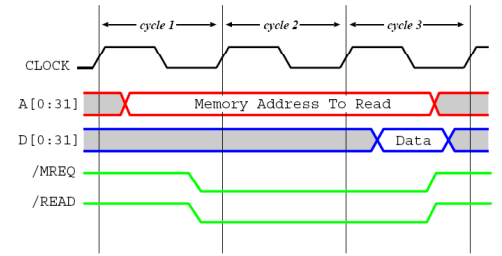
\includegraphics[width=8cm]{synchronousbus}
\end{center}

\newpage 

\item In what ways does an asynchronous bus differ?

Asynchronous buses do not have a master-slave configuration. Rather they use handshaking -- wherein 
the CPU sends a ready-signal, the device responds with a data-accept signal. This triggers the 
ready-signal to go low which in turn triggers to data-accept signal to go low. Data is then sent 
by the CPU to the device. The process is then reversed for sending the devices response to the 
CPU.

There is no bus clock so each device can send data as fast as they want -- this means that buffering 
is needed since one device may be faster than the other. Synchronous buses have a clock 
and do not require buffering.

\end{enumerate}

\end{enumerate}

\end{examquestion}

\end{document}